\chapter{Architettura e Struttura del Simulatore}
\label{cap:1}
L'instabilità intrinseca dell'F-16 e la forte non linearità delle sue equazioni del moto vengono rappresentate all' interno di questo simulatore che serve come strumento di validazione e per la linearizzazione e la validazione delle leggi di controllo che verranno create all'interni di questi capitoli Cap.\ref{cap:lqr} e Cap.\ref{cap:mpc}. Il simulatore è stato sviluppato in ambiente MATLAB/Simulink dal professore Raktim Bhattacharya \cite{bhattacharya_f16_trim}, adottando un approccio accademico e con una  organizzazione che permette di isolare i singoli fenomeni fisici (aerodinamica, cinematica, gravità, atmosfera).
\clearpage
\section{Panoramica Globale dell'Architettura}
La struttura principale del simulatore, riportata in Figura \ref{fig:simulink_full}, rappresenta il \textit{plant} del velivolo in anello aperto. Esso è composto da sei macro-blocchi interconnessi che si scambiano segnali cinematici e dinamici ad ogni istante di campionamento, risolvendo di fatto il sistema di equazioni differenziali ordinarie (ODE) che governa il moto nello spazio.

\begin{figure}[H]
	\centering
	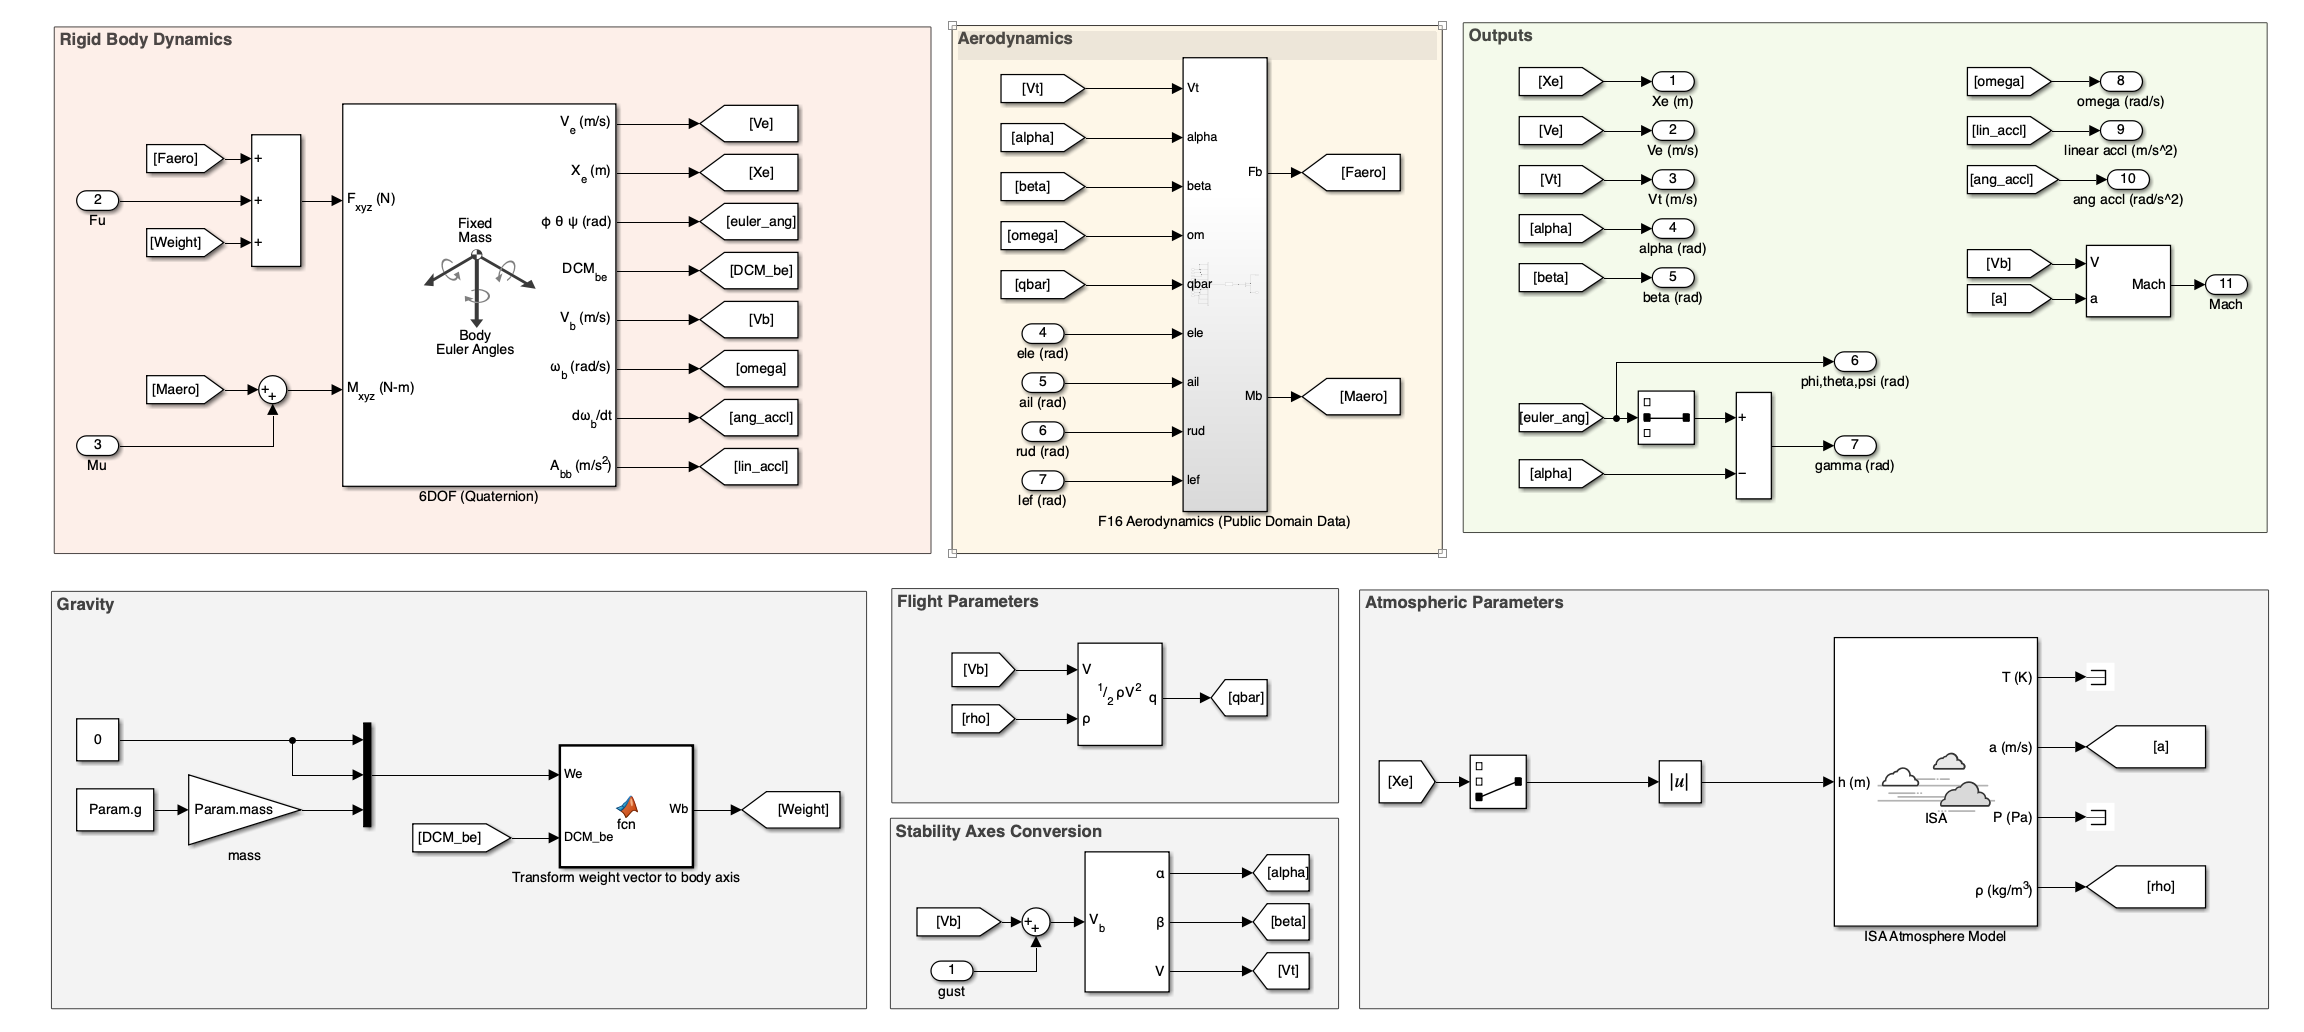
\includegraphics[width=1.0\textwidth]{Foto/simulatore.png}
	\caption{Architettura globale del simulatore F-16 in ambiente Simulink. Sono visibili i sei sottosistemi principali che governano la dinamica del volo.}
	\label{fig:simulink_full}
\end{figure}

Nelle sezioni seguenti verranno analizzati nel dettaglio i singoli sottosistemi, definendone gli ingressi, le uscite e le responsabilità computazionali all'interno del ciclo di simulazione.

% --- SOTTOSISTEMA 1: RIGID BODY DYNAMICS ---
\section{Dinamica del Corpo Rigido}


Il blocco \textbf{Rigid Body Dynamics} presente in \texttt{matlab} costituisce il nucleo cinematico del simulatore. Il suo scopo è integrare le equazioni di Newton-Eulero (che verranno discusse nel Capitolo \ref{sec:equazioni}) per propagare lo stato del velivolo nel tempo, pertanto, le equazioni differenziali non sono state implementate analiticamente riga per riga, bensì integrate direttamente tramite i solutori numerici di questo blocco Simulink.

\begin{figure}[H]
	\centering     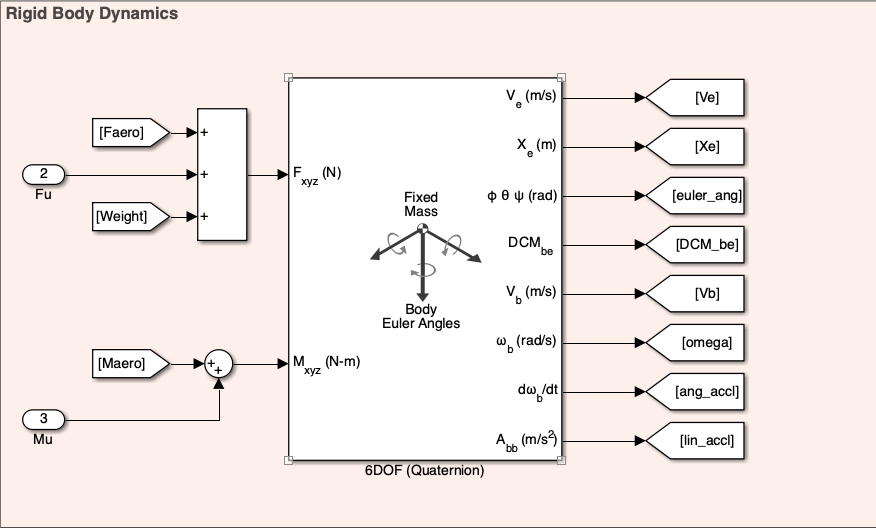
\includegraphics[width=0.7\textwidth]{Foto/RigidBodyDynamics.png}
	\caption{Dettaglio del blocco 6-DOF (Quaternion).}
\end{figure}

\begin{itemize}
	\item \textbf{Ingressi:} Il blocco riceve la sommatoria delle forze esterne applicate sul baricentro, composta dalle forze aerodinamiche (\texttt{Faero}) e dalla forza peso vettoriale (\texttt{Weight}). Parallelamente, riceve i momenti aerodinamici (\texttt{Maero}) generati dai ratei di rotazione e dalle superfici di controllo, questi valori vengono ottenuti utilizzando lo script MATLAB \texttt{F16AeroFM.m} (dettagliato nella Sezione \ref{F16AereoFM}), che computa le forze e i momenti risultanti.
	\item \textbf{Elaborazione:} Utilizza il blocco nativo di Simulink \textit{6DOF (Quaternion)}. L'integrazione numerica avviene sfruttando i parametri di Eulero (quaternioni) al fine di evitare le singolarità matematiche (\textit{Gimbal Lock}) tipiche del volo verticale che verranno trattati nel Capitolo \ref{sec:quaternioni}.
	\item \textbf{Uscite:}
	\label{DCM}
	Restituisce lo stato cinematico completo. Fornisce le velocità nel sistema corpo (\texttt{Vb}), le velocità e le posizioni nel sistema terrestre (\texttt{Ve}, \texttt{Xe}), gli angoli di Eulero classici per la telemetria (\texttt{euler\_ang}), i ratei angolari (\texttt{omega}) e le accelerazioni lineari e angolari e inoltre  Esporta la \textit{Direction Cosine Matrix} (\texttt{DCM\_be}), fondamentale per le proiezioni tra i sistemi di riferimento.
\end{itemize}

% --- SOTTOSISTEMA 2: AERODINAMICA ---
\section{Sottosistema Aerodinamico} 
Il blocco \textbf{Aerodynamics} funge da ponte tra la cinematica istantanea del velivolo e i dati sperimentali di galleria del vento che sono stati utilizzati per il calcolo dei coefficienti aerodinamici (Sezione \ref{sec:coefficienti_aerodinamici}, pubblicati nei database NASA).

\begin{itemize}
	
	\item \textbf{Ingressi:} L'aerodinamica dipende dalle variabili in ingresso ricevendo così la \textit{True Airspeed} (\texttt{Vt}), gli angoli di incidenza e derapata (\texttt{alpha}, \texttt{beta}), i ratei di rotazione (\texttt{omega}), la pressione dinamica (\texttt{qbar}) e, soprattutto, i comandi del pilota: deflessione di equilibratore (\texttt{ele}), alettoni (\texttt{ail}), timone (\texttt{rud}) e flap del bordo d'attacco (\texttt{lef}).
	
	
	\label{F16AereoFM}
	\item \textbf{Elaborazione:} Al suo interno viene richiamata la funzione MATLAB \texttt{F16AeroFM.m}. Questa funzione  interpola le tabelle dei coefficienti adimensionali, somma i contributi dei \textit{Leading Edge Flaps} e i termini di smorzamento, scalando infine i coefficienti mediante la geometria dell'ala per ottenere forze dimensionali in Newton.
	
	
	\item \textbf{Uscite:} Genera i vettori di forza aerodinamica (\texttt{Faero}) e momento aerodinamico (\texttt{Maero}) espressi nel Body Frame, che verranno inviati al solutore 6-DOF.
\end{itemize}

\vspace{0.5cm} % Piccolo spazio di respiro prima dell'immagine

\begin{figure}[H]
	\centering
	% Impostiamo un limite sia alla larghezza che all'altezza per evitare salti di pagina
	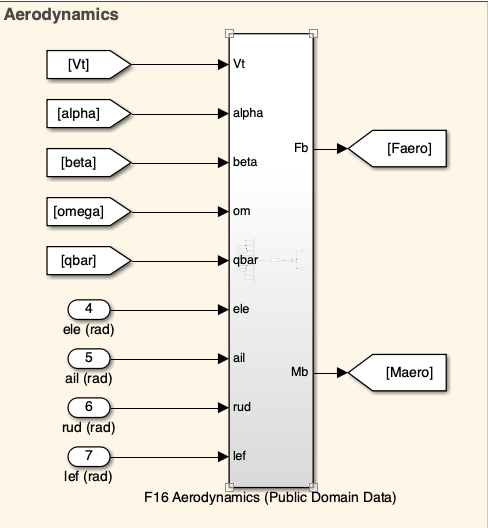
\includegraphics[width=0.8\textwidth, height=7.5cm, keepaspectratio]{Foto/Aerodinamica.png}
	\caption{Dettaglio del sottosistema Aerodinamico: interfaccia tra lo stato del velivolo e la funzione di calcolo dei coefficienti.}
	\label{fig:sub_aero}
\end{figure}

% --- SOTTOSISTEMA 3: PARAMETRI ATMOSFERICI ---
\section{Modello Atmosferico }
\label{blocco_atmosferico}
Le prestazioni dell' F-16 variano drasticamente in base alla quota di volo a causa delle variazioni di densità e temperatura dell'aria. Questo blocco modella l'ambiente in cui il velivolo si muove.

\begin{itemize}
	\item \textbf{Ingressi:} Riceve la posizione inerziale del velivolo (\texttt{Xe}), estraendo specificamente la terza componente cambiata di segno, ovvero la quota altimetrica geometrica $h$, l'equazione usata per descrivere questa varibaile si trova al Capitolo \ref{eqAltitudine}.
	\item \textbf{Elaborazione:} Implementa il modello \textit{ISA (International Standard Atmosphere)}. Calcola i gradienti termici e barometrici in base all' altitudone a cui si trova l'aereo.
	\item \textbf{Uscite:} Fornisce al sistema la temperatura assoluta $T$, la velocità del suono locale $a$, la pressione statica $P$ e la densità dell'aria $\rho$. Quest'ultima è un parametro critico per la determinazione della portanza.
\end{itemize}

\begin{figure}[H]
	\centering
	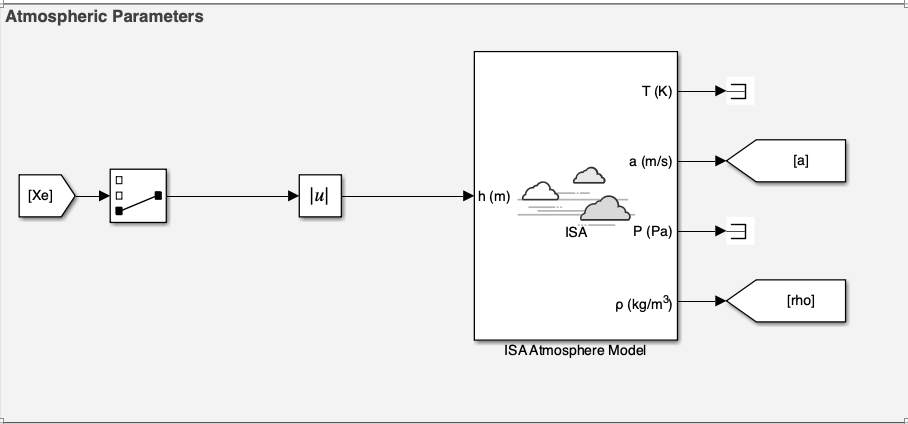
\includegraphics[width=0.85\textwidth]{Foto/Atmosphere.png}
	\caption{Implementazione del modello atmosferico ISA per il calcolo dei parametri ambientali in funzione della quota.}
	\label{fig:sub_atmo}
\end{figure}

% --- SOTTOSISTEMA 4: PARAMETRI DI VOLO ---
\section{Parametri di Volo e Assi di Stabilità }

Questa sezione del modello calcola le variabili aerodinamiche secondarie necessarie alla simulazione.

\begin{itemize}
	\item \textbf{Conversione agli Assi di Stabilità:} Riceve il vettore velocità letto nel Body Frame (\texttt{Vb}) e lo scompone. In tale sezione è predisposto un nodo di somma (\texttt{gust}) che permette l'iniezione di modelli stocastici di raffiche di vento per valutare la robustezza del velivolo. Infine, l'uscita fornisce l'angolo d'attacco $\alpha$, l'angolo di derapata $\beta$ e la velocità totale $V_t$.
	\item \textbf{Pressione Dinamica:} Sfruttando la velocità $V_t$ appena calcolata e la densità $\rho$ proveniente dal modello atmosferico e calcola la pressione dinamica $\bar{q} = \frac{1}{2} \rho V_T^2$. Questo segnale viene poi instradato verso il blocco aerodinamico.
\end{itemize}

\begin{figure}[H]
	\centering
	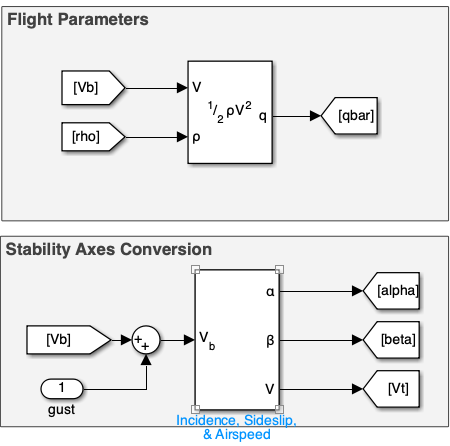
\includegraphics[width=0.75\textwidth]{Foto/FlightParameters.png}
	\caption{Sottosistema per il calcolo delle variabili cinematiche $\alpha$, $\beta$ e della pressione dinamica $q$.}
	\label{fig:sub_flight_params}
\end{figure}

% --- SOTTOSISTEMA 5: GRAVITÀ ---
\section{Modellazione della Gravità }

Il calcolo della forza peso richiede particolare attenzione poiché l'integrazione dinamica avviene in un sistema rotante e solidale all'aereo (Body Frame).

\begin{itemize}
	\item \textbf{Logica:} Nel sistema di riferimento terrestre (NED), il vettore peso ha una sola componente attiva diretta verso il basso, pari a $[0, 0, m \cdot g]^T$ come presente inoltre all'interno del modello \texttt{matlab}.
	\item \textbf{Elaborazione:} Il blocco riceve la massa costante del velivolo moltiplicata per l'accelerazione di gravità $g$. Utilizzando la matrice di rotazione \texttt{DCM\_be} presa dal locco alla sezione \ref{DCM} nella sezione delle \texttt{Uscite}, calcolata dal blocco 6-DOF e poi proiettata istantaneamente il  vettore gravità negli assi inerziali agli assi corpo.
	\item \textbf{Uscita:} Il vettore \texttt{Weight} risultante, che alle elevate incidenze o durante i rollii si distribuisce sugli assi $X_{body}$ e $Y_{body}$ influenzando pesantemente la dinamica longitudinale e laterale.
\end{itemize}

All'interno del sottosistema è presente un blocco \textit{MATLAB Function} che esegue materialmente il prodotto matriciale. Il codice implementato riceve il vettore peso inerziale (\texttt{We}) e la \textit{Direction Cosine Matrix} (\ref{DCM}) (\texttt{DCM\_be}), restituendo il vettore proiettato negli assi corpo (\texttt{Wb}):

\begin{lstlisting}[language=MATLAB, caption={Proiezione vettoriale della forza peso tramite blocco MATLAB Function.}]
	function Wb = fcn(We, DCM_be)
	Wb = DCM_be * We; % Weight in body coordinate system. 
	% DCM_be is correct, no need for transpose. They must have fixed it in this version.
\end{lstlisting}

\begin{figure}[H]
	\centering
	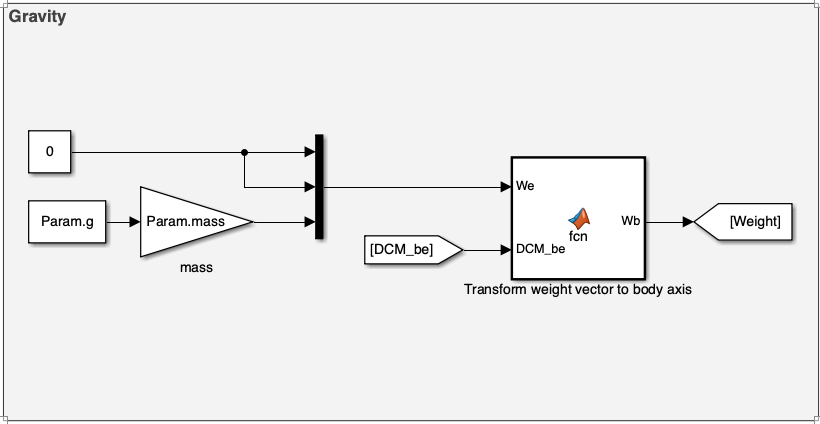
\includegraphics[width=0.6\textwidth]{Foto/Gravity.png}
	\caption{Trasformazione vettoriale della forza peso dal sistema NED agli assi corpo tramite Direction Cosine Matrix.}
	\label{fig:sub_gravity}
\end{figure}

% --- SOTTOSISTEMA 6: USCITE ---
\section{Condizionamento delle Uscite }

Tale blocco ha lo scopo di condizionare i segnali di uscita destinati al motore di rendering visivo FlightGear (trattato nel Capitolo \ref{cap2}. Oltre a riordinare i flussi dei bus il blocco esegue due calcoli derivati essenziali:
\begin{enumerate}
	\item \textbf{Numero di Mach:} Calcolato come rapporto tra la velocità relativa (\texttt{Vb}) e la velocità del suono locale ($a$) fornita dal blocco atmosferico \ref{blocco_atmosferico}.
	\item \textbf{Angolo di Rampa (Flight Path Angle, $\gamma$):} Estrae l'angolo di beccheggio $\theta$ dal vettore di Eulero e vi sottrae l'angolo d'attacco $\alpha$. Il parametro $\gamma = \theta - \alpha$.
\end{enumerate}

\begin{figure}[H]
	\centering
	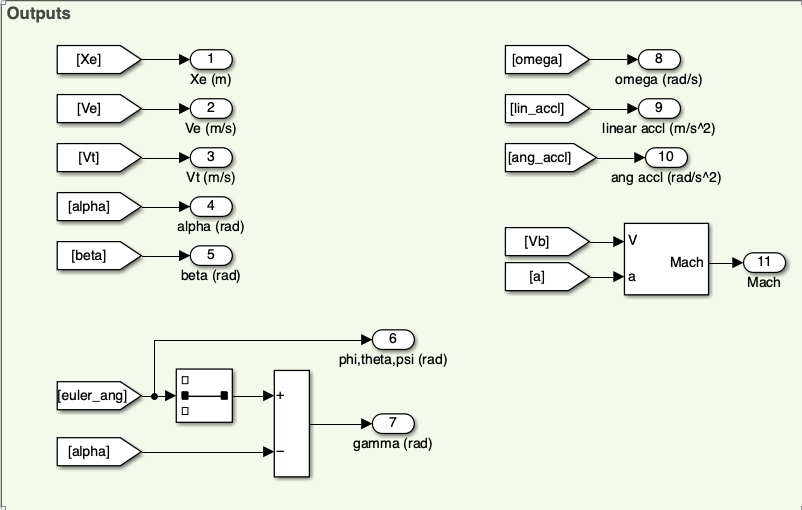
\includegraphics[width=0.65\textwidth]{Foto/Outputs.png}
	\caption{Condizionamento dei segnali di uscita e calcolo dei parametri di volo derivati (Mach, Gamma).}
	\label{fig:sub_outputs}
\end{figure}

%Capitolo 2 Simulatore Matlab F-16
